%NYU 2019 Grad Computational Physics Homework 2

\documentclass[12pt, graphicx]{article}
\pagestyle{plain}
\baselineskip 18pt
\textwidth 6.5in
\textheight 7.8in
\oddsidemargin 0.1in
\evensidemargin 0.1in
\topmargin 0.3in
\parindent 0pt
\linespread{1.5}
\setlength{\parskip}{2.5mm}

\usepackage{graphicx, psfrag, epsfig}
\usepackage[font = small, format = plain, labelfont = bf, textfont = it, justification = raggedright, singlelinecheck = false]{caption}
\usepackage{subfig}
\usepackage{amsmath, amssymb}
\usepackage{geometry}
%\usepackage[symbol]{footmisc}

\renewcommand\tablename{Table}
\renewcommand\figurename{Fig.}
\renewcommand{\thefootnote}{\fnsymbol{footnote}}


\begin{document}
\title{Computational Physics Homework 2}
\author{Hao Li\footnotemark[2]}
\footnotetext[2]{hl3270@nyu.edu~~UID:N12137527}
\date{\today}


\maketitle

\section*{Problem 1}
\subsection*{a)}
The true solution is related to the current estimate $x$ and the next estimate $x'$ of the equation is 
\begin{equation}
\begin{gathered}
x^*=(1+\omega)f(x^*)-\omega x^*\\
x^*=x+\epsilon\\
x^*=x'+\epsilon'
\end{gathered}
\label{eq1}
\end{equation} 
Here $\epsilon$ and $\epsilon'$ are the error on the two estimates. Then Taylor expand the iteration function of the overrelaxation function about the true solution $x^*$
\begin{equation}
x'=(1+\omega)f(x)-\omega x=(1+\omega)[f(x^*)+(x-x^*)f'(x^*)]-\omega x
\label{eq2}
\end{equation}
Now plug Eq. \ref{eq1} into Eq. \ref{eq2}, we will get 
\begin{equation}
x'-x^*=(1+\omega)[x^*+(x-x^*)f'(x^*)]+(x-x^*)-(1+\omega)x=(x-x^*)[(1+\omega)f'(x^*)-\omega]
\end{equation}
that is
\begin{equation}
\epsilon'=\epsilon[(1+\omega)f'(x^*)-\omega]
\end{equation}
Back to Eq. \ref{eq1}
\begin{equation}
x^*=x+\epsilon=x+\frac{\epsilon'}{(1+\omega)f'(x^*)-\omega}=x'+\epsilon'
\end{equation}
So the equivalent of Eq. (6.83) for the overrelaxation method is 
\begin{equation}
\epsilon'\approx\frac{x-x'}{1-\frac{1}{(1+\omega)f'(x)-\omega}}
\label{eq4}
\end{equation}
\subsection*{b)}
To calculate $x=1-\mathrm{e}^{-cx}$, $c=2$ with relaxation method, the iteration function is simply 
\begin{equation}
x'=1-\mathrm{e}^{-cx}
\label{eq3}
\end{equation}
The code for relaxation method to solve (nonlinear) equations is available in \textquotedblleft relaxation.h\textquotedblright, attached in the folder. By inputing the starting point $x_0$ and the target accuracy of solution, the code returns the final answer $x$ and the process of iteration. Here we set the starting point to be $x_0=1$, and the desired accuracy to be $10^{-6}$. It takes 13 steps to converge to an accuracy better than the target, and the solution $x$ by the program and the true solution $x^*$ by Mathematica to Eq. \ref{eq3} are
\begin{equation}
\begin{gathered}
x=0.796812(7)\\
x^*=0.79681213
\end{gathered}
\end{equation}
So the error $\epsilon\approx7\times10^{-7}<10^{-6}$. The solution given by the program reaches the desired accuracy. The process of iteration is shown in Figure. \ref{fig:rel}. 

\begin{figure}[ht]
\centering
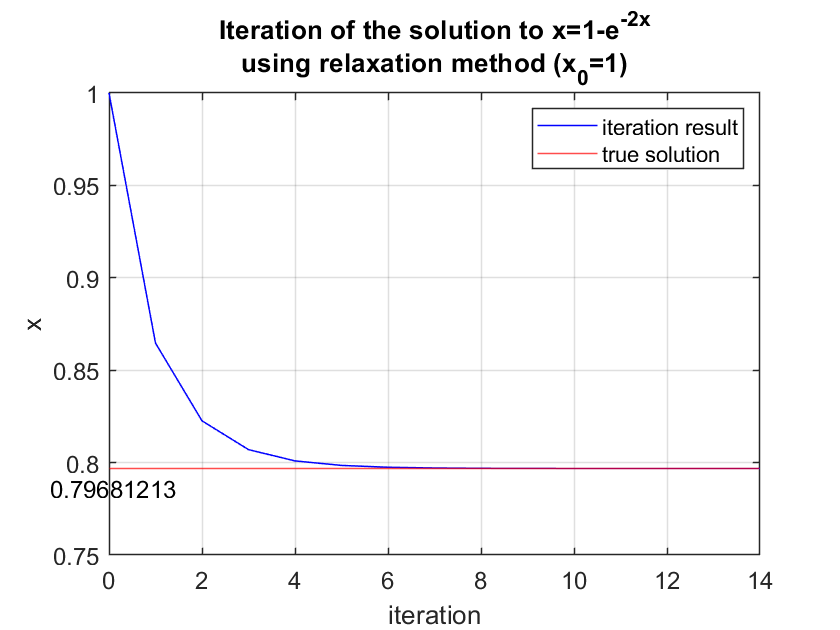
\includegraphics[width = 120mm]{relaxation.png}
\caption{The iteration process of the solution to $x=1-\mathrm{e}^{-2x}$ using relaxation method. Starting from $x_0=1$, and target accuracy $\epsilon=10^{-6}$}
\label{fig:rel}
\end{figure}

\subsection*{c)}
According to Eq. \ref{eq2}, the overrelaxation iteration equation is 
\begin{equation}
x'=(1+\omega)(1-\mathrm{e}^{-2x})-\omega x
\end{equation}
The code for overrelaxation method to solve (nonlinear) equations is available in \textquotedblleft relaxation.h\textquotedblright, attached in the folder. By inputing the starting point $x_0$ and the target accuracy of solution, the code returns the final answer $x$ for different parameter $\omega$, and the number of iterations for each $\omega$ with other conditions the same. Here we still set the starting point to be $x_0=1$, and the desired accuracy to be $10^{-6}$. From Figure. \ref{fig:overrel} we can see that there is an range of optimal value of $\omega$ about $[0.5,0.7]$ that can converge twice or three times faster than the standard relaxation method. 

\begin{figure}[ht]
\centering
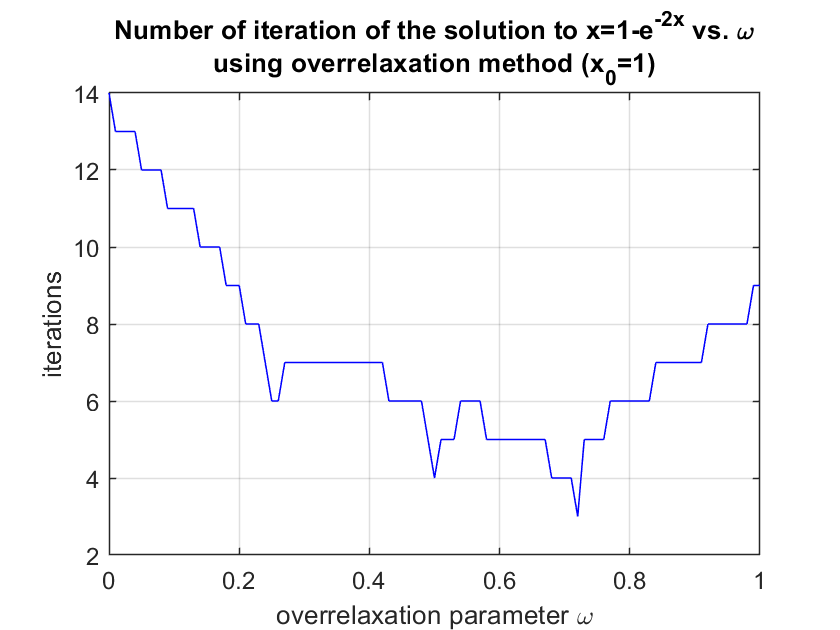
\includegraphics[width = 120mm]{overrelaxation.png}
\caption{The number of iterations of the solution to $x=1-\mathrm{e}^{-2x}$ using overrelaxation method, with respect to the overrelaxation parameter $\omega$. Starting from $x_0=1$, and target accuracy $\epsilon=10^{-6}$, parameter $\omega\in[0,1]$.}
\label{fig:overrel}
\end{figure}

The stop condition of the iteration is the error estimated by Eq. \ref{eq4}, replacing the derivative with the finite estimate 
\begin{equation}
\epsilon'\approx\dfrac{x-x'}{1-\dfrac{1}{(1+\omega)\dfrac{(f(x)-f(x'))}{x-x'}-\omega}}<\epsilon_\mathrm{tar}
\label{eq5}
\end{equation}
The final results for all $\omega$'s are plotted in Figure. \ref{fig:overresult} with respect to $\omega$. From the plot we can see that for most of the values of $\omega\in[0,1]$, the error is just as estimated using Eq. \ref{eq5}, except for a narrow range arround [0.2,0.3], there is a spike whose error $\epsilon\sim10^{-5}$. So the break condition of the code may need further improvement.

\begin{figure}[ht]
\centering
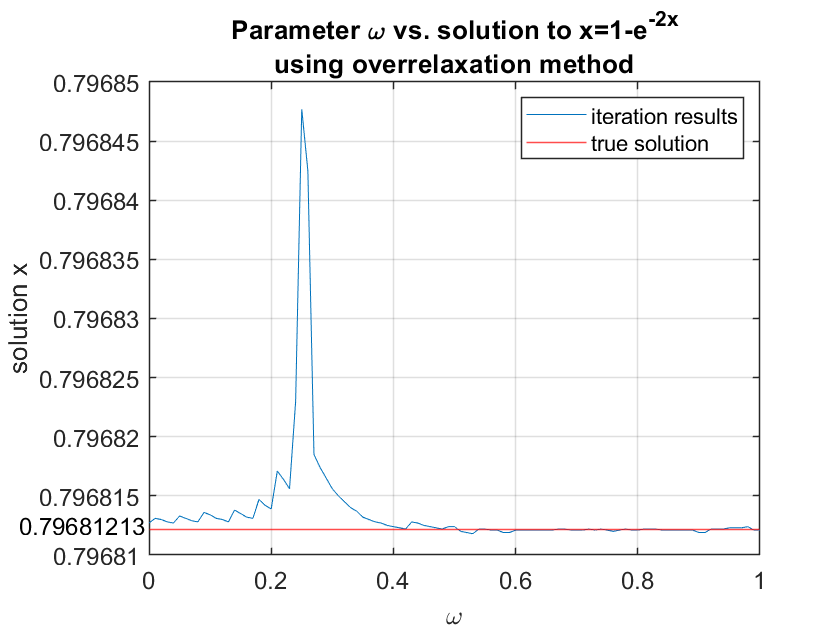
\includegraphics[width = 120mm]{overresult.png}
\caption{The iteration solution to $x=1-\mathrm{e}^{-2x}$ using overrelaxation method, with respect to the overrelaxation parameter $\omega$. $x_0=1$, target accuracy $\epsilon=10^{-6}$, parameter $\omega\in[0,1]$.  For most of the values of $\omega\in[0,1]$, the error is just as estimated using Eq. \ref{eq5}, except for a narrow range arround [0.2,0.3], there is a spike whose error $\epsilon\sim10^{-5}$.}
\label{fig:overresult}
\end{figure}

\subsection*{d)}
From Eq. \ref{eq4}, we can see that if we expect an $\omega<0$ could help speed up 
\begin{equation}
|(1+\omega)f'(x)-\omega|<|f'(x)|
\end{equation}
The solutions are $f'(x^*)>1$ or $-1<f'(x^*)<0$. For $f'(x^*)>1$, we can modify $\omega$ so that the solution could converge. For $-1<f'(x^*)<0$, the underrelaxation method $\omega<0$ could help converge faster compared with standard relaxation method.

\section*{Problem 2}
\subsection*{a)}
The intensity of radiation from a black body 
\begin{equation}
I(\lambda)=\frac{2\pi hc^2\lambda^{-5}}{\mathrm{e}^{hc/\lambda k_BT}-1}
\end{equation}
The first derivative with respect to wavelenth $\lambda$
\begin{equation}
\frac{\mathrm{d}I(\lambda)}{\mathrm{d}\lambda}=\frac{2\pi hc^2\lambda^{-6}\mathrm{e}^{hc/\lambda k_BT}}{(\mathrm{e}^{hc/\lambda k_BT}-1)^2}[5(\mathrm{e}^{-hc/\lambda k_BT}-1)+\frac{hc}{\lambda k_BT}]
\end{equation}
For the wavelenth $\lambda$ at which the emmited radiation is strongest, there should be $\frac{\mathrm{d}I(\lambda)}{\mathrm{d}\lambda}=0$, i.e. 
\begin{equation}
5(\mathrm{e}^{-hc/\lambda k_BT}-1)+\frac{hc}{\lambda k_BT}=0
\end{equation}
Substitute $x=hc/\lambda k_BT$, then the equation is 
\begin{equation}
5\mathrm{e}^x+x-5=0
\label{eq6}
\end{equation}
Define the Wien displacement constant $b=hc/k_Bx$, where $x$ is the solution to Eq. \ref{eq6}, then from the substitution we can derive the Wien displacement law 
\begin{equation}
\lambda=\frac{hc}{k_BxT}=\frac{b}{T}
\label{eq7}
\end{equation}

\subsection*{b)}
The program to solve the Eq. \ref{eq6} is available in \textquotedblleft root\_finding.h\textquotedblright, attched in the folder. Starting with the interval $[x_1,x_2]=[4,6]$, with an accuracy of $\epsilon=10^{-6}$, as shown in Figure. \ref{fig:bin}, the root of the equation is 
\begin{equation}
x=4.965114
\end{equation}
which agrees with the true solution 
\begin{equation}
x^*=4.9651142317
\end{equation}

\begin{figure}[ht]
\begin{minipage}{0.48\linewidth}
\centering
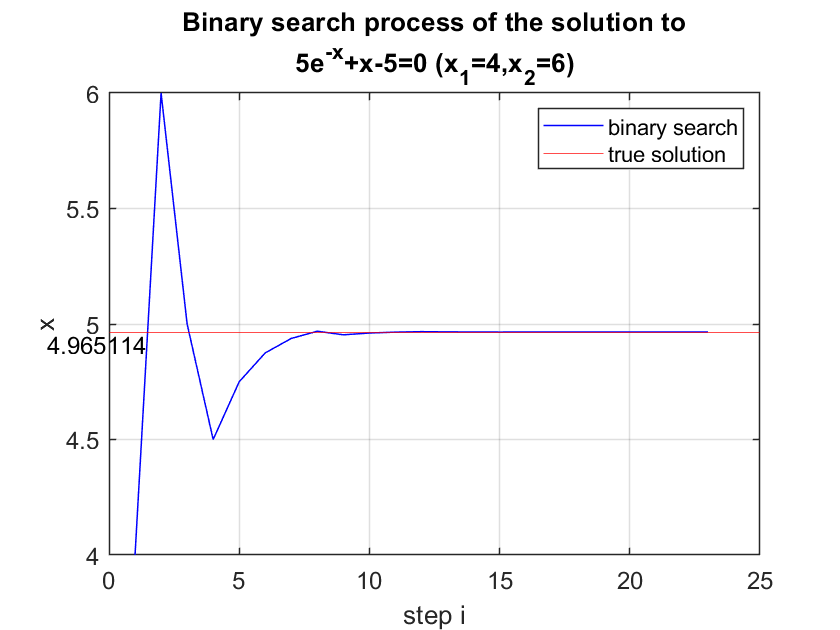
\includegraphics[width = 80mm]{binary_search.png}
\end{minipage}
\begin{minipage}{0.48\linewidth}
\centering
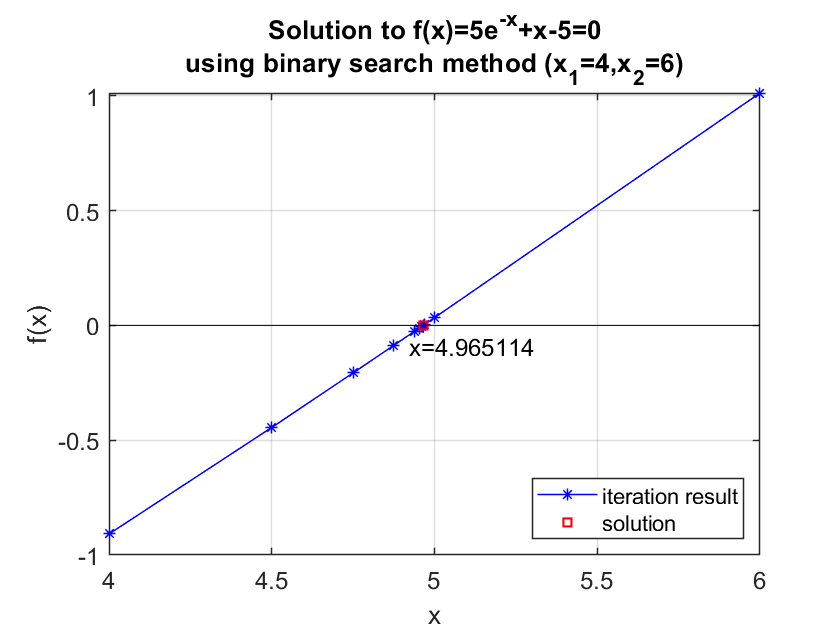
\includegraphics[width = 80mm]{binary_result.png}
\end{minipage}
\caption{The binary search process and result of solution to the equation $5\mathrm{e}^{-x}+x-5=0$. Starting with the interval $[x_1,x_2]=[4,6]$, target accuracy $\epsilon=10^{-6}$. The solution given by the program is $x=4.965114$, which agrees with the true solution.}
\label{fig:bin}
\end{figure}

\subsection*{c)}
From Eq. \ref{eq7} we have 
\begin{equation}
T=\frac{b}{\lambda}=\frac{hc}{k_Bx\lambda}
\end{equation}
Plug in the result in b) and $\lambda=5.2\mathrm{nm}$, an estimate for the tempreture of the Sun is 
\begin{equation}
T\approx5.77\times10^3\mathrm{K}
\end{equation}

\section*{Problem 3}
\subsection*{a)}
To find the minimum of a multi dimensional function $f(\mathbf{x})$ using the gradient descent method, we start from an initial position $\mathbf{x}_0$, $f(\mathbf{x})$ decreases fastest in the negative gradient $\nabla f(\mathbf{x})$. That is, for small enough step size $\gamma$ 
\begin{equation}
\mathbf{x}_{n+1}=\mathbf{x}_n-\lambda\nabla f(\mathbf{x_n})
\label{eq8}
\end{equation}
gives $f(\mathbf{x}_{n+1})<f(\mathbf{x}_n)$. For complecated or unknown expression function, we use numerical derivatives  to calculate the gradient and plug in Eq. \ref{eq8}. The loop stops when the maximum difference in $\mathbf{x}$ (or some other difference) reaches the target accuracy. \par
For further usage in fitting the Schechter function, first test the code on a simple function
\begin{equation}
f(x,y)=(x-2)^2+(y-2)^2
\label{eq9}
\end{equation}
The code that implement the gradient descent method to find the minimum of a multi dimensional function, using numerical derivatives, is available in \textquotedblleft descent.h\textquotedblright. By inputing the function $f(\mathbf{x})$ and its dimension, the initial position $\mathbf{x}_0$, step size $\gamma$, the target accuracy $\epsilon$, and the maximum number of loops to avoid infinite calculation, the code saves the process of calculation and returns the final result. \par
For the simple function Eq. \ref{eq9}, two initial points $(x_0,y_0)=(0,1), (3,1)$ with two step sizes $\gamma=10^{-2},10^{-3}$, and accuracy $\epsilon=10^{-7}$, are tested respectively to see if the final solution is the same. \par
Figure. \ref{fig:testxy} shows that different initial points with different step sizes will give the same result within some error range. The four results of the four initial conditions are (1.999995,1.999997), (1.999950,1.999970), (2.000006,1.999997), (2.000059,1.999970), are clearly the correct results $(x,y)=(2,2)$ in a relatively high accuracy. 

\begin{figure}[ht]
\begin{minipage}{0.48\linewidth}
\centering
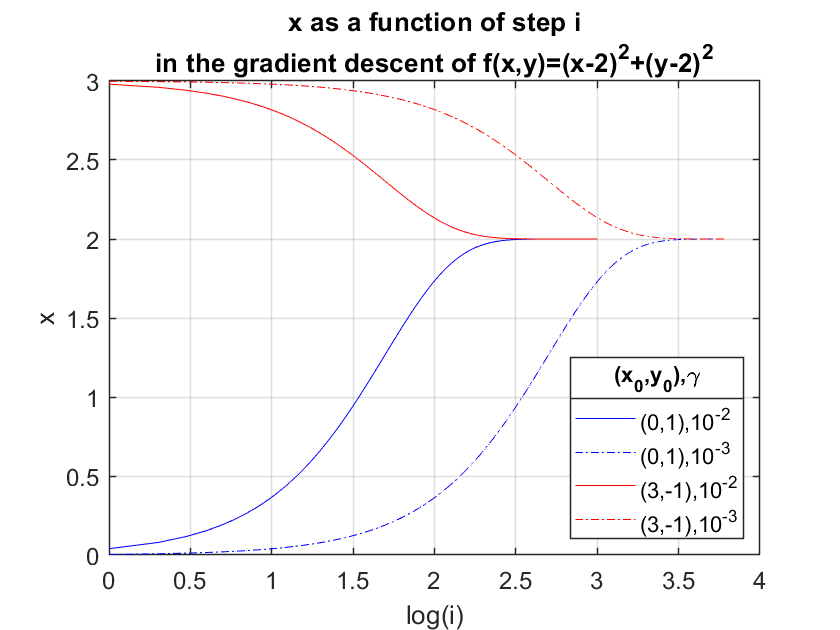
\includegraphics[width = 80mm]{test_x.png}
\end{minipage}
\begin{minipage}{0.48\linewidth}
\centering
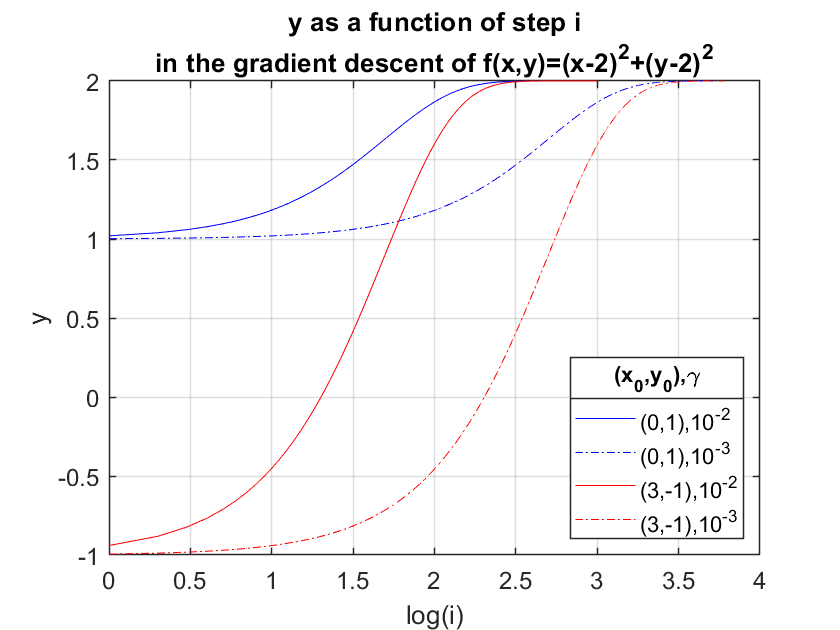
\includegraphics[width = 80mm]{test_y.png}
\end{minipage}
\caption{Finding the minimum of the function $f(x,y)=(x-2)^2+(y-2)^2$ using gradient descent method.  Initial points $(x_0,y_0)=(0,1), (3,1)$, step sizes $\gamma=10^{-2},10^{-3}$, accuracy $\epsilon=10^{-7}$. it confirms that the code can give the same result with different initial conditions,  and is thus robust within at least a small vincinity of the true minimum.}
\label{fig:testxy}
\end{figure}

The evolution of the position and the function value in the four processes above are given in Figure. \ref{fig:test}. From the test result, it is obvious that the code is robust within at least a small vincinity of the true minimum. 

\begin{figure}[ht]
\begin{minipage}{0.48\linewidth}
\centering
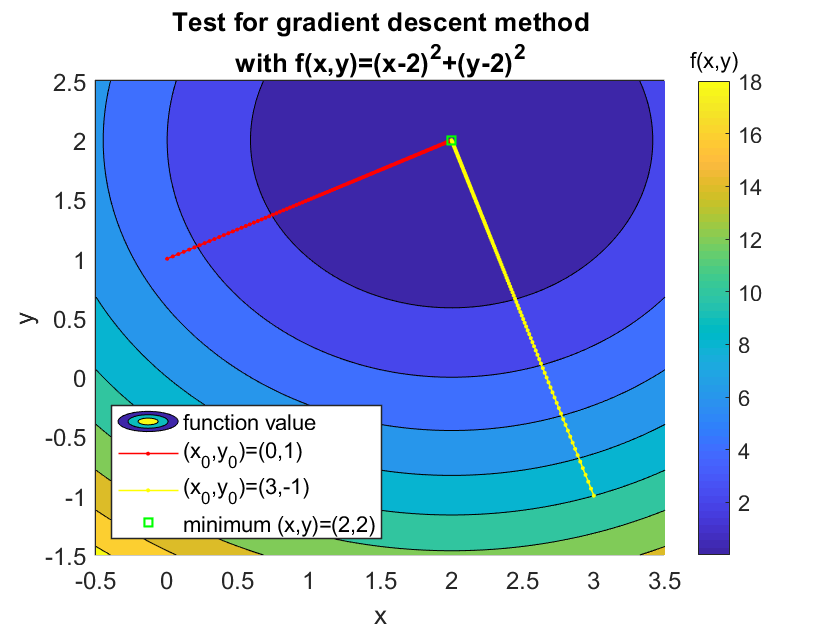
\includegraphics[width = 80mm]{grad_test.png}
\end{minipage}
\begin{minipage}{0.48\linewidth}
\centering
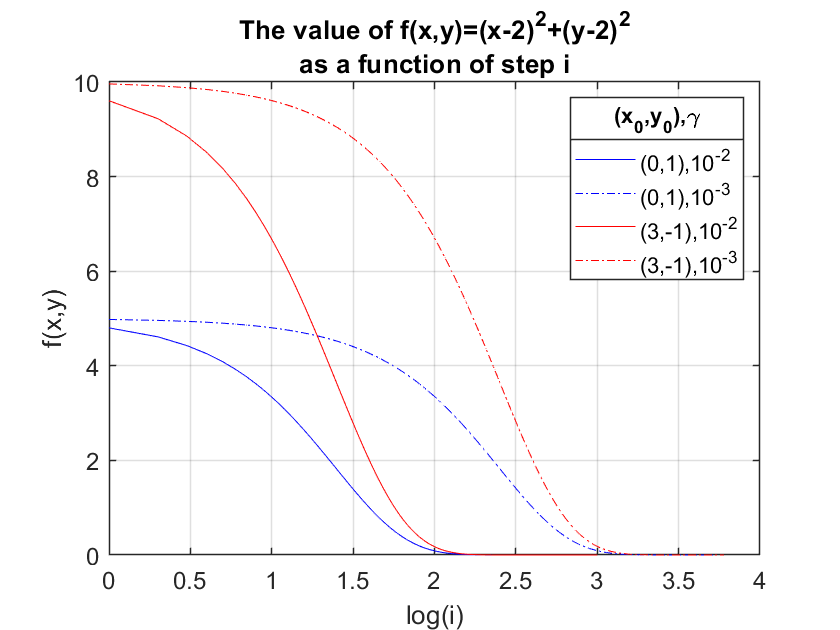
\includegraphics[width = 80mm]{test_value.png}
\end{minipage}
\caption{The evolution of the position $(x,y)$ and the value of the function $f(x,y)=(x-2)^2+(y-2)^2$ in the gradient descent process, with initial points $(x_0,y_0)=(0,1), (3,1)$, step sizes $\gamma=10^{-2},10^{-3}$, and accuracy $\epsilon=10^{-7}$. it is obvious that he four different initial conditions will lead to the same true minimum, thus confirms the robustness of the code.}
\label{fig:test}
\end{figure}

\subsection*{b)}
Now that the code works, it is going to be applied to the problem of fitting the Schechter function
\begin{equation}
n(M_\mathrm{gal})=\phi^*\left(\frac{M_\mathrm{gal}}{M^*}\right)^{\alpha+1}\mathrm{exp}\left(-\frac{M_\mathrm{gal}}{M^*}\right)\ln(10)
\end{equation}
From the data file \textquotedblleft smf\_cosmos.dat\textquotedblright we can see that $M_\mathrm{gal}$ is rather large while $n(M_\mathrm{gal})$ is small. And it can be guessed that the exponent $\alpha$ cannot be large, so the variables used in fitting are $\log(\phi^*)$, $\log(M^*)$, and $\alpha$ since they are close to 1. \par
Guessing from the data, four initial points are chosen to verify the robustness of the code: $(\log(\phi^*),\log(M^*),\alpha)=(-5,9.5,-1.5),(-3,10.5,-1),(-3,10,0),(-4,9,-0.5)$. Step size are the same $\gamma=10^{-4}$, and the target accuracy $\epsilon=2\times10^{-7}$. \par
The function to minimize is the $\chi^2$ of the model
\begin{equation}
\chi^2=\displaystyle\sum_{i=1}^N\left(\frac{n_{i,\mathrm{fit}}-n_{i,\mathrm{data}}}{\sigma}\right)^2
\end{equation}
The evolution of the three parameters $(\log(\phi^*),\log(M^*),\alpha)$ are as given in Figure. \ref{fig:para}. And the final result of the fitting is 
\begin{equation}
\begin{gathered}
\log(\phi^*)=-2.5682(1)\\
\log(M^*)=10.9762(3)\\
\alpha=-1.0093(9)
\end{gathered}
\end{equation}
The minimum $\chi^2$ is 
\begin{equation}
\chi^2=2.90806(5)
\end{equation}
The evolution of $\chi^2$ as  a function of $i$ is shown in Figure. \ref{fig:chi2}.

\begin{figure}[ht]
\begin{minipage}{0.48\linewidth}
\centering
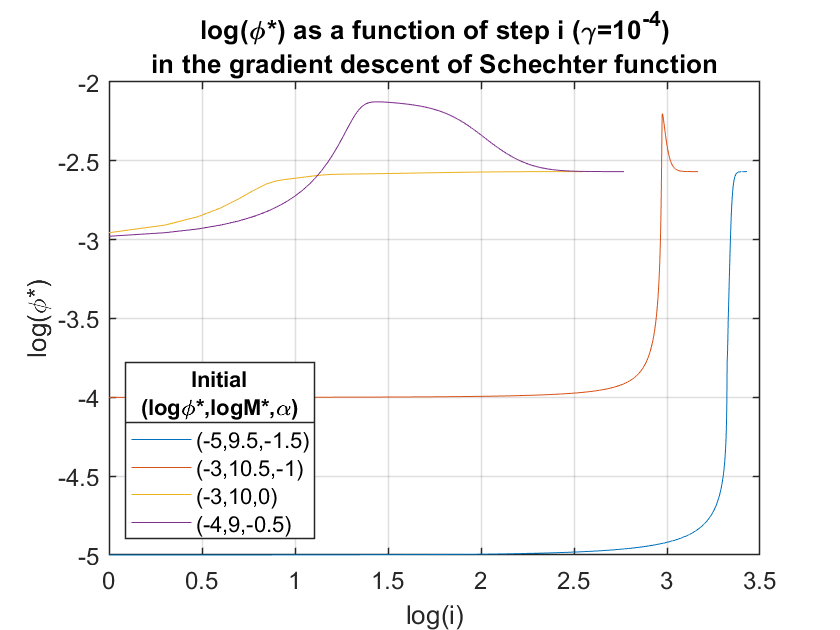
\includegraphics[width = 80mm]{phi.png}
\end{minipage}
\begin{minipage}{0.48\linewidth}
\centering
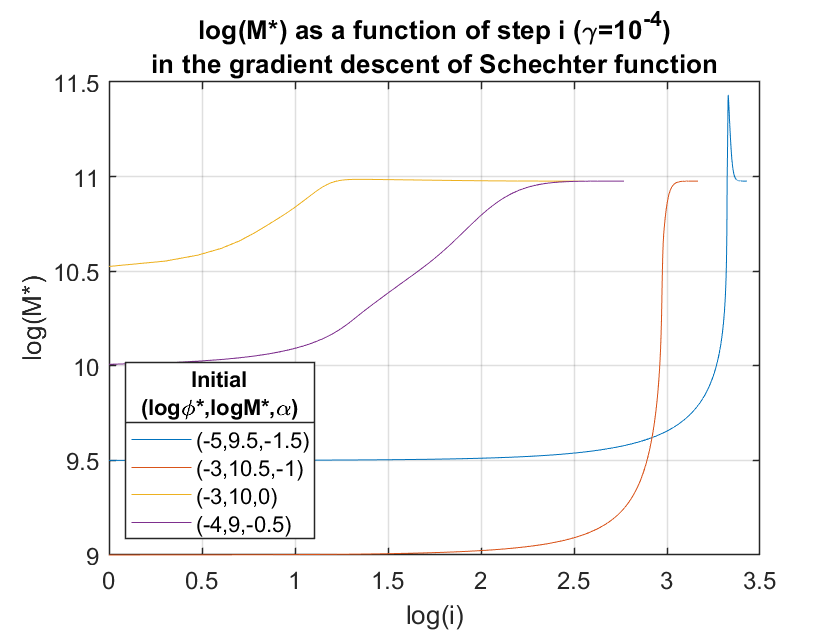
\includegraphics[width = 80mm]{m.png}
\end{minipage}
\centering
\begin{minipage}{0.48\linewidth}
\centering
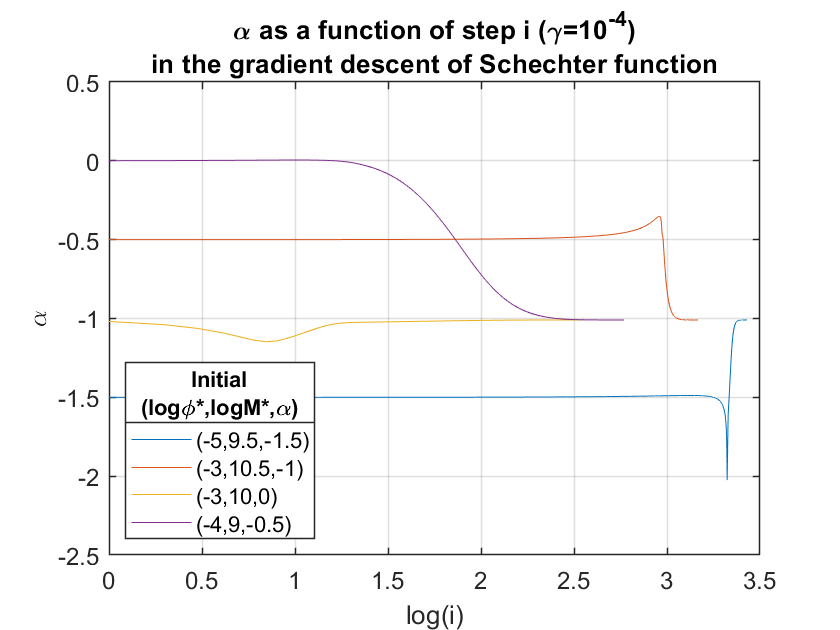
\includegraphics[width = 80mm]{alpha.png}
\end{minipage}
\caption{The evolution of the parameters $(\log(\phi^*),\log(M^*),\alpha)$. Initial points $(\log(\phi^*),\log(M^*),\alpha)=(-5,9.5,-1.5),(-3,10.5,-1),(-3,10,0),(-4,9,-0.5)$, and accuracy $\epsilon=10^{-7}$. The results are all $(-2.5682,10.9762,-1.0094)$ with high accyracy of about $10^{-5}$, thus demonstrating that the result is robust.}
\label{fig:para}
\end{figure}

\begin{figure}[ht]
\centering
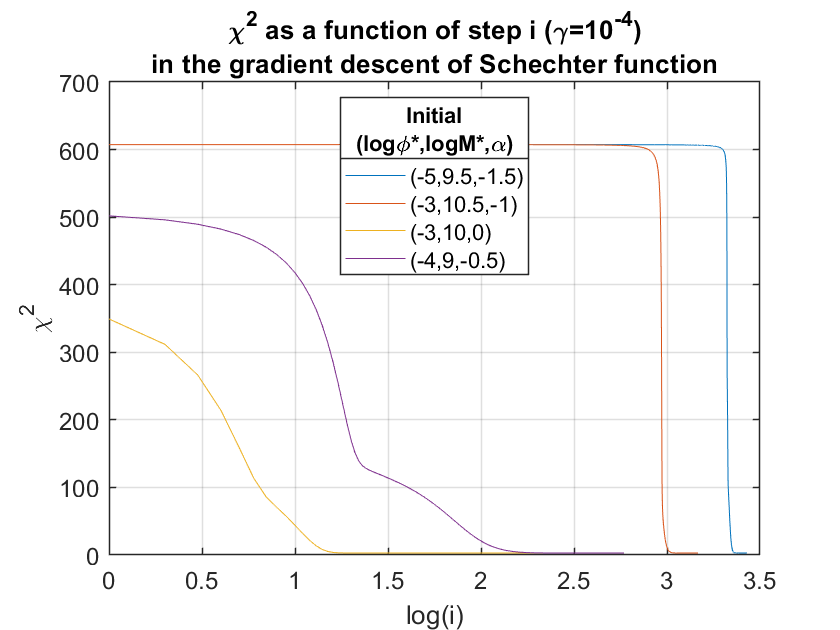
\includegraphics[width = 120mm]{chi2.png}
\caption{$\chi^2$ of the Schechter function as a function of step $i$. Initial points $(\log(\phi^*),\log(M^*),\alpha)=(-5,9.5,-1.5),(-3,10.5,-1),(-3,10,0),(-4,9,-0.5)$, and accuracy $\epsilon=10^{-7}$. The results are all $(-2.5682,10.9762,-1.0094)$ with high accyracy of about $10^{-5}$, thus demonstrating that the result is robust.}
\label{fig:chi2}
\end{figure}

However, it can be seen from Figure. \ref{fig:para} and \ref{fig:chi2} that for initial points far from the minimum, the value of the variables and the function might stay nearly unchanged for quite a few steps, may be because it is far, and may be because the derivative may be close to zero, i.e. the function is nearly flat. In this circumstance, it will take exponentially longer time to finish calculation and converge to the minimum. In practice, when starting with $\log(M_\mathrm{gal})\approx14$, or $\alpha\approx1$, it may remain unconverged in over 8000 steps, with $\chi^2$ or some parameters staying nearly the same , so I am not sure if it could work for arbitrary initial points in single precision. \par
Finally, Figure. \ref{fig:fit} shows the comparison of the best-fit Schechter function to the data in log-log plot. The fit result agrees quite well with the data. 

\begin{figure}[ht]
\centering
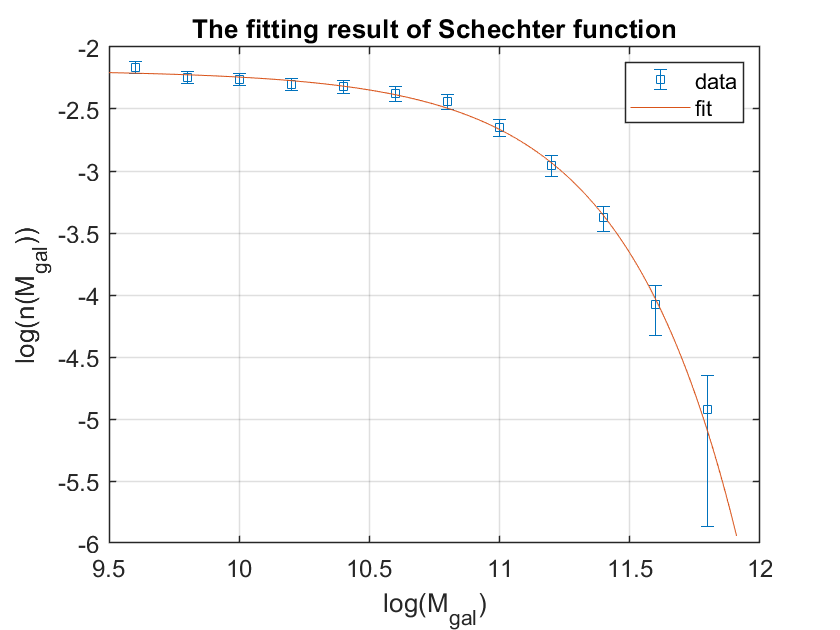
\includegraphics[width = 120mm]{fit.png}
\caption{The comparison of the best-fit Schechter function to the data in log-log plot.}
\label{fig:fit}
\end{figure}



\end{document}